\begin{itemize}
    \item
        U und I bei verschiene Lasten, siehe Pflichtenheft.
            ==> Kurven plotten (gemessen und berechnet).
    \item
        Transienten, Laständerungen
    \item
        Leistungsaufnahme
    \item
        Dings funktioniert nicht
    \item
        Structure:
            1) Definition of test fixture
            2) What we actually did
            3) Error analysis
\end{itemize}


There are a variety of tests that can be conducted to verify the performance and
correctness of our  device.  The  following is a list of test fixtures and their
expected results based on simulations.

\subsection{Test Fixtures}

\subsubsection{Simple VI Curve}


\subsubsection{Non-Simple VI Curve}


\subsubsection{Ripple Voltage and Ripple Current vs Resistive Load}

\begin{figure}[th!]
    \centering
    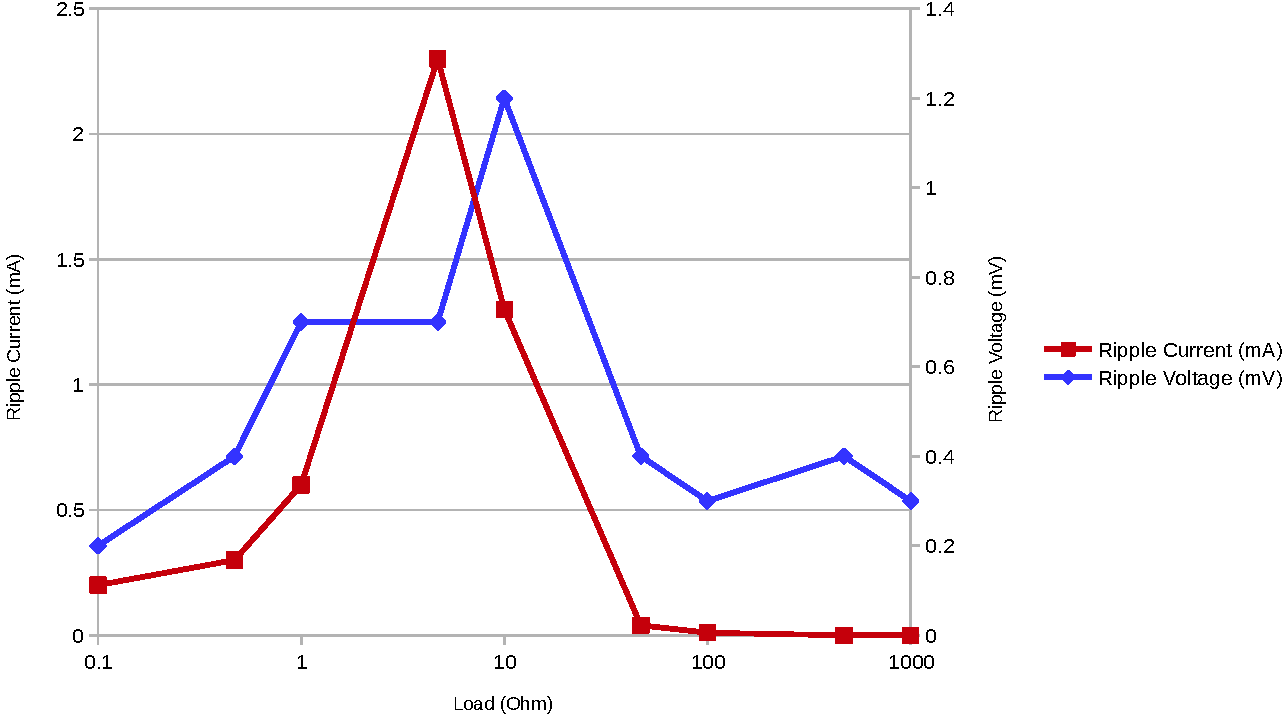
\includegraphics[width=.7\textwidth]{images/sim/ripple-vs-load.pdf}
    \caption{Simulation of the amplitude of the ripple voltage and ripple current vs different resistive loads, obtained using LTSpiceIV's model of the LT3741}
\end{figure}


\subsubsection{Power Absorbtion}


\subsubsection{Transient Response}


\subsubsection{Inductive Load}


\subsection{Measurement Results}

Unfortunately, we were unable to  operate the LT3741 for a period long enough to
conduct any of the measurements listed above.  The same regulator model (LT3741)
was  permanently  damaged  twice  in  a row. Please see the next section  for  a
detailed analysis on what we think the issue is and how we would proceed if more
time were available.


\subsection{Analysis of the Issue}

\subsubsection{A Quick Overview}

The first regulator output the  correct  voltage  of  \SI{12}{\volt}  when being
supplied with \SI{32}{\volt}.  Unplugging  the  device and re-plugging it into a
\SI{36}{\volt}  power  supply  instantly  damaged  it  permanently.  After  some
detailed measurements (a more detailed description of  these measurements can be
found in the next section) it was concluded that the high-side driver inside the
LT3741 was somehow damaged  and  not  operating as it should. Our assumption was
that -- since we were operating the device very  closely  to its maximum ratings
of  \SI{40}{\volt} -- during switching, the high-side MOSFET driver was  exposed
to transients exceeding the device's absolute maximum  ratings and thus damaging
the driver permanently.

The  regulator  was  replaced with a new one and the supply voltage was  lowered
from \SI{36}{\volt} to \SI{28}{\volt} in order  to  give  more  leeway  for  the
supposed transient voltages. The new  regulator  appeared  to output the correct
voltage of  \SI{12}{\volt}.  A  resistive load of \SI{80}{\ohm} was connected on
the output  of  the  regulator.  After  about  \SI{20}{\second}  of  continuous
operation,  the  output  voltage  again  dropped and the device was  permanently
damaged. Unfortunately, we were unable to capture some vital measurements of the
transients we were looking for to confirm our suspicions from the first failure.


\subsection{Detailed Analysis}


